\title[Alignment of Recordings with Study Materials]{Automatic alignment of Lecture Recordings with Study Materials}
\mode<presentation>{\subtitle[github.com/video699]{\color{black}\faGithub\ \href{https://github.com/video699}{github.com/video699}}}
\author[V.\,Novotný]{Vít Novotný, witiko@mail.muni.cz}
\year=2018\month=11\day=26
\institute[FI MU]{Faculty of Informatics, Masaryk University}
\subject{Research project report}
\keywords{information retrieval, image processing, pattern recognition, machine learning}

\begin{document}
\begin{frame}[plain]
\maketitle
\begin{tikzpicture}[overlay,remember picture]
    \node[anchor=south east, xshift=-38pt, yshift=20pt] at (current page.south east) {
      \includegraphics[width=70mm]{figs/gnus-gnats/recording}
    };
\end{tikzpicture}
\end{frame}

% \begin{frame}{Contents}
% \begin{multicols}{2}
% \tableofcontents
% \end{multicols}
% \end{frame}

\section{Introduction}

\begin{frame}{Introduction \titlenote{\cite[sec.~1]{novotny18}}}
\begin{itemize}
\item<1-7> \abbr{FI} \abbr{MU} has been \alert{recording lectures} and publishing the
  recordings since 2004~\cite{hladkaliska03lectures}.
\item<3-7> Two years of knowledge are archived with \alert{no indexing} and
  \alert{no metadata}.
\item<4-7> \abbr{SPEECH@FIT} use \alert{speech recognition} to annotate videos at
  \href{https://superlectures.com/}{superlectures.com}.
\item<5-7> We use \alert{digital image processing} to map recordings to lecture
  materials.
\item<7> We published our system, and datasets under \alert{open licenses}
  at \href{https://github.com/video699}{github.com/video699}.
\end{itemize}

\begin{center}
\only<1>{\vspace{-2cm}\includegraphics[height=0.7\textheight]{figs/gnus-gnats/lecture-01}}
\only<2>{\vspace{-3.5cm}\includegraphics[height=0.82\textheight]{figs/gnus-gnats/storage}}
\only<3>{\vspace{-1.8cm}\includegraphics[height=0.65\textheight]{figs/franek/overload}}
\only<4>{\vspace{-1.8cm}\includegraphics[height=0.7\textheight]{figs/gnus-gnats/search-results}}
\only<5>{\vspace{-1cm}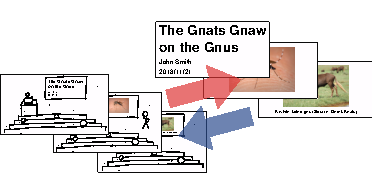
\includegraphics[height=0.6\textheight]{figs/gnus-gnats/mapping}}
\only<6>{\vspace{-1.8cm}\includegraphics[height=0.7\textheight]{figs/gnus-gnats/search-results}}
\only<7>{%
  \includegraphics[height=0.4\textheight]{figs/logo/gplv3}%
  \hspace{1cm}
  \includegraphics[height=0.4\textheight]{figs/logo/ok}%
}
\end{center}

\end{frame}

\section{Tasks}

\begin{frame}{Tasks \titlenote{\cite[sec.~2.2]{novotny18}}}
\begin{itemize}
\item<1-5> Given a \alert{lecture recording} and a set of \alert{lecture materials},
  we need to produce a set of \alert{time segments} during which the recording
  displays a lecture material.
\item<2-5> We break this high-level task into \alert{four elementary subtasks}:
\begin{description}
\item<2-5>[\task{FRAMES}] Detect \alert{significant video frames}, where
  lecture materials transition.
\item<3-5>[\task{SCREENS}] Detect \alert{projection screens} in a significant
  video frame.
\item<4-5>[\task{RETRIEVAL}] Find the \alert{nearest lecture materials} to a
  projection screen.
\item<5-5>[\task{CLASSIFICATION}] Decide if nearest lecture materials
  \alert{match} the projection screen.
\end{description}
\end{itemize}

\begin{center}
\only<1>{\vspace{-3cm}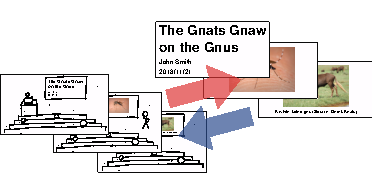
\includegraphics[height=0.7\textheight]{figs/gnus-gnats/mapping}}%
\only<2>{\vspace{-1.5cm}\hspace{3cm}\includegraphics[height=0.53\textheight]{figs/gnus-gnats/frames}}%
\only<3>{\vspace{-1.9cm}\includegraphics[height=0.6\textheight]{figs/gnus-gnats/screens}}%
\only<4>{\vspace{-1.9cm}\includegraphics[height=0.6\textheight]{figs/gnus-gnats/retrieval}}%
\only<5>{\vspace{-0.1cm}\includegraphics[height=0.3\textheight]{figs/gnus-gnats/matching}}%
\end{center}
\end{frame}

\section{System}

\begin{frame}{
  System \titlenote{%
    \autocites[sec.~4]{novotny18}{research-system}{implementation-system}{video699}%
  }%
}
\begin{itemize}
\item<1-6> We built our system~\cite{implementation-system} in \alert{Python 3.4}
  using the following C++ libraries:
\begin{description}
\item<1-6>[\library{Annoy}] A library for \alert{approximate nearest neighbor
  retrieval}.
\item<1-6>[\library{spatialindex}] A library for \alert{spatial indexing}.
\item<1-6>[\library{GEOS}] A library for \alert{computational geometry}.
\item<2-6>[\library{MuPDF}] An \alert{AGPL-licensed} library for \alert{rendering
  \abbr{PDF}, and \abbr{XPS} documents}.
\item<3-6>[\library{TensorFlow}] A library for \alert{building neural networks}.
\end{description}
\item<4-6> Here is how our system solves the individual \alert{subtasks}:
\begin{description}
\item<4-6>[\task{FRAMES}] We currently \alert{process all video frames}.
\item<5-6>[\task{SCREENS}] We \alert{use our dataset}~\cite{implementation-screens}
  to detect projection screens.  We implemented tracking of screen movements in
  \library{spatialindex}, and \library{GEOS}.
\item<6-6>[\task{RETRIEVAL}\bodytext{, }\task{CLASSIFICATION}] We implemented a supervised
  method using \alert{Siamese convolutional neural networks}~\cite{bromley94}
  in \library{Annoy}, and \library{TensorFlow}.
\end{description}
\end{itemize}
\end{frame}

\begin{frame}
\begin{figure}
\begin{center}
\includegraphics[width=1.47\textheight, height=0.9\textheight]{figs/diagramm/bromley94}
\end{center}
\vspace{-0.3cm}%
\caption{A Siamese convolutional neural network. Source: \textcite{bromley94}}
\end{figure}
\end{frame}

\section{Datasets}

\begin{frame}{Datasets \titlenote{\cite[sec.~3]{novotny18}}}
\begin{itemize}
\item<1-11> We need a dataset~\cite{implementation-videos} for
  \alert{supervised learning} to \alert{evaluate} our system:
\begin{itemize}
\item<1-11> We collected a random sample of \alert{17 lecture recordings} from 2010--2016.
\item<2-11> We drew a stratified sample of \alert{up to 25 video frames} from each recording.
\item<4-11> In each frame, we annotated \alert{lit projection screens} and
  their condition.
\item<6-11> For each lit projection screen, we annotated \alert{lecture materials} shown in
  the screen.
\item<8-11> The dataset contains \alert{699 projection screen annotations}, and
  \alert{925 lecture materials}.
\end{itemize}
\item<9-11> We need a dataset~\cite{implementation-screens} to solve
  \task{SCREENS}:
\begin{itemize}
\item<9-11> We annotated \alert{three rooms} at \abbr{FI MU}.
\item<10-11> In each room, we anotated \alert{camcoders}, and \alert{projection screens}.
\item<11-11> We annotated \alert{positions of screens} in the coordinates of
  every camcoder across time.
\end{itemize}
\end{itemize}

\begin{center}
\only<1,2,4,6,8-11>{%
  \vspace{-2cm}
  \only<1>{%
    \includegraphics[width=2\textwidth]{figs/diagramm/implementation-dataset_videos}%
  }%
  \only<2>{%
    \hspace*{-3cm}%
    \includegraphics[width=2\textwidth]{figs/diagramm/implementation-dataset_frames}%
  }%
  \only<4>{%
    \hspace*{-6.5cm}%
    \includegraphics[width=2\textwidth]{figs/diagramm/implementation-dataset_screens}%
  }%
  \only<6>{%
    \hspace*{-14cm}%
    \includegraphics[width=2\textwidth]{figs/diagramm/implementation-dataset_keyrefs}%
  }%
  \only<8>{%
    \vspace{0.35cm}
    \hspace*{-15cm}%
    \includegraphics[width=2\textwidth]{figs/diagramm/implementation-dataset_keyref_page}%
  }%
  \only<9>{%
    \includegraphics[width=2\textwidth]{figs/diagramm/implementation-screens_rooms}%
  }%
  \only<10>{%
    \hspace*{-3cm}%
    \includegraphics[width=2\textwidth]{figs/diagramm/implementation-screens_camcoders_screens}%
  }%
  \only<11>{%
    \hspace*{-14.5cm}%
    \includegraphics[width=2\textwidth]{figs/diagramm/implementation-screens_positions}%
  }%
}%
\only<3>{%
  \vspace{-2cm}\leavevmode
  \includegraphics[width=0.3\textwidth]{implementation-videos/PA152-D3-20110331.avi/frame002000}
  \includegraphics[width=0.3\textwidth]{implementation-videos/PA152-D3-20110331.avi/frame004000}
  \includegraphics[width=0.3\textwidth]{implementation-videos/PA152-D3-20110331.avi/frame006000}%
}%
\only<5>{%
  \vspace{-2.2cm}\leavevmode
  \includegraphics[align=c, width=0.3\textwidth]{figs/dataset-examples/beyond-bounds/frame004000}
  \includegraphics[align=c, width=0.3\textwidth]{figs/dataset-examples/beyond-bounds/frame004000-00}
  \includegraphics[align=c, width=0.3\textwidth]{figs/dataset-examples/beyond-bounds/frame004000-01}%
}%
\only<7>{%
  \vspace{-2cm}\leavevmode
  \includegraphics[width=0.3\textwidth]{figs/dataset-examples/beyond-bounds/frame004000-00}
  \includegraphics[width=0.3\textwidth]{figs/dataset-examples/beyond-bounds/frame004000-01}
  \includegraphics[width=0.3\textwidth]{figs/dataset-examples/beyond-bounds/slides01-12}%
}%
\end{center}
\end{frame}

\section{Evaluation and Results}

\begin{frame}{Evaluation and Results \titlenote{\cite{siamese-cnn-evaluation}}}
\begin{itemize}
\item We estimated the system's \alert{performance} on \task{RETRIEVAL}, and
  \task{CLASSIFICATION}:
\begin{itemize}
\item We used \alert{\abbr{CV}} to split videos in the dataset into \alert{training and validation sets}.
\item We produced \alert{image pairs} of projection screens, and lecture materials.
\item We trained the Siamese neural network to correctly \alert{classify the image pairs}.
\end{itemize}
\end{itemize}

\begin{center}
\vspace{-0.2cm}%
\includegraphics[width=\textwidth]{figs/results/siamese-21}
\end{center}
\end{frame}

\section{Conclusion and Future Work}

\begin{frame}{Conclusion and Future Work}
\begin{itemize}
\item<1-7> In our project, we have accomplished the following:
\begin{itemize}
\item<1-7> We have developed a \alert{production-grade system} and \alert{two
  datasets} and released them under open licenses.
\item<2-7> We have proposed and evaluated a \alert{novel method} for content-based
  image retrieval and image pair classification using \alert{modern digital
  image processing techniques}.
\end{itemize}
\item<3-7> In the future, we will focus on the following:
\begin{itemize}
\item<3-7> Solving \task{FRAMES} is expected to \alert{improve the speed} of our system.
\item<4-7> Solving \task{SCREENS} will \alert{automate projection screen detection}.
\item<5-7> Removing \alert{uneven illumination}, \alert{noise}, and \alert{optical
  distortion} from video frames is expected to \alert{improve the accuracy} of our system.
\item<6-7> Optimizing \alert{hyper-parameters} is expected to \alert{improve
  both speed and accuracy}.
\item<7-7> We will deploy our system at \href{https://video.muni.cz/}{video.muni.cz}.
\end{itemize}
\end{itemize}
\end{frame}

\section{Acknowledgements}

\begin{frame}{Acknowledgements I}
\begin{itemize}
\item<1-3> Computational resources \alert{hypnos} were kindly provided by
  \alert{the Laboratory of Electronic and MultiMedia Applications}
  (\alert{\abbr{LEMMA}}).
\item<2-3> Access to pre-trained \abbr{VGG} convolutional neural networks was
  kindly provided by
  \alert{RNDr.\ David Novák},
  \alert{Ph.D., RNDr.\ Michal Batko, Ph.D.}, and
  \alert{Mgr.\ Michal Lukáč}
  from \alert{the Laboratory of Data Intensive Systems and Applications}
  (\alert{\abbr{DISA}}).
\item<3-3> We would like to thank
  \alert{Doc.\ RNDr.\ Petr Sojka, Ph.D.}, 
  \alert{doc.\ RNDr.\ Petr Matula, Ph.D.},
  \alert{RNDr.\ David Novák, Ph.D.}, and
  \alert{doc.\ Ing.\ Vlad Popovici, Ph.D.}\ for useful feedback.
\end{itemize}

\begin{center}%
\only<1>{\vspace{-2.3cm}\includegraphics[width=0.3\textwidth]{figs/logo/lemma}}%
\only<2>{\vspace{-2.2cm}\includegraphics[width=\textwidth]{figs/logo/disa}}%
\only<3>{\vspace{6cm}}%
\end{center}%
\end{frame}

\begin{frame}{Acknowledgements II}
We would like to acknowledge the following lecturers, listed in no particular
order, who kindly agreed to have their lecture recordings and lecture
materials released in a public dataset. Their contribution to this work is
gratefully acknowledged.

\scriptsize
\begin{multicols}{3}
\begin{itemize}
\item\alert{RNDr.\ Václav Brožek, Ph.D.},
\item\alert{RNDr.\ Nikola Beneš, Ph.D.},
\item\alert{doc.\ Mgr.\ Radek Pelánek, Ph.D.},
\item\alert{prof.\ RNDr.\ Petr Hliněný, Ph.D.},
\item\alert{doc.\ RNDr.\ Jan Bouda, Ph.D.},
\item\alert{prof.\ RNDr.\ Jan Slovák, DrSc.},
\item\alert{RNDr.\ Radek Ošlejšek, Ph.D.},
\item\alert{doc.\ RNDr.\ Vlastislav Dohnal, Ph.D.},
\item\alert{prof.\ RNDr.\ Luděk Matyska, CSc.},
\item\alert{doc.\ RNDr.\ Eva Hladká, Ph.D.},
\item\alert{prof.\ Ing.\ Jiří Sochor, CSc.},
\item\alert{doc.\ RNDr.\ Petr Sojka, Ph.D.},
\item\alert{Jeffrey Dean, Ph.D.},
\item\alert{Bc.\ Jakub Hančin},
\item\alert{RNDr.\ Jaroslav Pelikán, Ph.D.},
\item\alert{RNDr.\ Jan Kasprzak, Ph.D.},
\item\alert{doc.\ RNDr.\ Barbora Kozlíková, Ph.D.},
\item\alert{Mgr.\ Petr Tobola, Ph.D.}
\end{itemize}
\end{multicols}
\end{frame}

\section{Bibliography}

\begin{frame}[allowframebreaks]{Bibliography}
\printbibliography
\end{frame}
\end{document}
